\documentclass[12pt]{article}
\usepackage[paper=letterpaper,margin=2cm]{geometry}
\usepackage{enumitem}
\usepackage{amsmath}
\usepackage{graphicx}
\usepackage{xcolor}
\usepackage{tabularray}
\usepackage{mathtools}

\graphicspath{ {./images/} }
\setlength{\parindent}{0pt}

\begin{document}

\begin{titlepage}
    \begin{center}
        \vspace*{1cm}

        \textbf{Redes de Computadores}
        \vspace{0.5cm}

        Resumo
        \vspace{1.5cm}

        \textbf{Rafael Rodrigues}
        \vfill
        LEIC \\
        Instituto Superior Técnico \\
        2022/2023
    \end{center}
\end{titlepage}

\tableofcontents

\newpage

\section{Introduction}

\subsection{What is a Protocol?}
A protocol defines the format and the order of messages exchanged between two or more communicating entities, as
well as the actions taken on the transmission and/or receipt of a message or other event.
\begin{itemize}
    \item Hardware-implemented Protocol → Controls the flow of bits on the 'wire' between the 2 network cards.
    \item Congestion-Control Protocol → Controls the rate at which packets are transmitted between sender and receiver.
    \item Router Protocol → Determines a packet's path from source to destination.
\end{itemize}

\subsection{Network Edge}

\subsection{Network Core}

\subsubsection{Packet Switching}

\begin{itemize}
    \item Comunicação dividida em pacotes, que partilham recursos com os restantes utilizadores.
    \item Cada um usa a largura de banda toda do canal. Recursos usados quando necessários.
    \item Não há alocação de canais.
\end{itemize}

\subsubsection{Circuit Switching}

\begin{itemize}
    \item Reserva largura de banda em todo o percurso, somo se ligasse cabos fisicamente.
    \item Precisa de setup, não há partilha de recursos.
    \item Garantias de performance. 
\end{itemize}

\subsubsection*{Packet Switching vs Circuit Switching}

Packet Switching é excelente para comunicação bursty, cujas necessidade de recursos varia com o tempo.

\subsection{Performance Metrics}

\subsection{Protocol Layers}

To provide structure to the design of network protocols, network designers organize them in layers.

Each layer provides its service by (1) performing certain actions within
that layer and by (2) using the services of the layer directly below it. \\

Advantage → Layering provides a structured way to discuss system components. \\
Disadvantage → One layer may duplicate lower-layer functionality. \\

\newpage

\section{Application Layer}

The application layer is where network applications and their application-layer protocols reside. The Internet's application layer includes many protocols, such as the HTTP protocol (which provides for Web document request and transfer), SMTP (which provides for the transfer of e-mail messages), and FTP (which provides for the transfer of files between two end systems). We'll see that certain network functions, such as the translation of human-friendly names for Internet end systems like www.ietf.org to a 32-bit network address, are also done with the help of a specific application-layer protocol, namely, the domain name system (DNS). We'll see in Chapter 2 that it is very easy to create and deploy our own new application-layer protocols.
\vspace{0.5cm} \\
An application-layer protocol is distributed over multiple end systems, with the application in one end system using the protocol to exchange packets of information with the application in another end system. We'll refer to this packet of information at the application layer as a message.

\subsection{Principles of Network Applications}

\subsubsection{Network Application Architectures}

\begin{itemize}
    \item Client-Server Architecture:
        \begin{itemize}[topsep=0pt]
            \item Um host (servidor) para vários hosts (clientes).
            \item Servidor sempre ligado, com endereço IP permanente.
            \item Clientes não precisam de estar conectados continuamente, podem utilizar IPs dinâmicos.
            \item Clientes não comunicam diretamente entre eles.
            \item Escalável com server farms.
        \end{itemize}
    \item P2P Architecture:
        \begin{itemize}[topsep=0pt]
            \item Não há servidor sempre ligado, peers comunicam entre si diretamente.
            \item Peers não precisam de estar conectados continuamente e podem mudar de IP.
            \item Bastante escalável, mas díficil de gerir.
        \end{itemize}
    \item Híbrido \\
        Exemplo do Skype: Servidor dá aos clientes os endereços, mas chamadas voz são feitas diretamente entre os clientes utilizando uma aplicação Voice-over-IP P2P.
\end{itemize}

\subsubsection{Processes Communicating}

\subsection{The Web and HTTP [Port 80]}

É o protocolo da Camada de Aplicação usado na WWW (World Wide Web), usando o protocolo TCP da Camada de Transporte. Existem várias versões:

\begin{itemize}
    \item HTTP 1.0
        \begin{itemize}[topsep=0pt]
            \item Versão não persistente.
            \item Cada objeto transferido exige a criação e uso de uma sessão de TCP diferente.
        \end{itemize}
    \item HTTP 1.1
        \begin{itemize}[topsep=0pt]
            \item Versão persistente, permitindo a transferência de vários objetos na mesma sessão de TCP.
            \item Permite pipelining - se existem referências a um dado objeto numa dada transferência, o cliente pode pedi-los imediatamente, em vez de ter de esperar pela resposta de um pedido antes de fazer o próximo.
        \end{itemize}
    \item HTTP 2.0
        \begin{itemize}[topsep=0pt]
            \item redução dos overheads dos cabeçalhos (são usados códigos para representar o conteúdo dos pedidos e respostas).
            \item permite que várias tabs de um dado browser partilhem a mesma ligação TCP.
            \item \textbf{Server Push}: O servidor analisa o HTML e vê que outros ficheiros são necessários (e consequentemente, serão pedidos) e envia-os assim que possível, não sendo necessário um pedido por parte do utilizador.
            \item \textbf{Mitigação de HOL blocking}: Os objetos são divididos em pacotes e a transferência é intercalada, de forma a transmitir os ficheiros mais pequenos primeiro.
        \end{itemize}
    \item HTTP 3.0
        \begin{itemize}[topsep=0pt]
            \item Invés do protocolo de comunicação, usa-se o protocolo QUIC - mistura do protocolo UDP com algumas diferenças e com encriptação.
        \end{itemize}
\end{itemize}

\subsubsection{Non-Persistent and Persistent Connections}

\begin{itemize}
    \item Non-Persistent Connection: \\
        Cada par pedido/resposta é feito numa ligação TCP diferente.
        \begin{itemize}[topsep=0pt]
            \item 2 RTT por objeto HTML. 
            \item $2+2N\ RTT$
        \end{itemize}
    \item Persistent Connection: \\
        Todos os pares pedido/resposta são feitos na mesma ligação TCP.
        \begin{itemize}[topsep=0pt, itemsep=0pt]
            \item 2 RTT para o primeiro objeto HTML.
            \item 1 RTT para os restantes objetos.
            \item $2+N\ RTT$
        \end{itemize}
\end{itemize}

Com pipelining:

\begin{itemize}[topsep=0pt, itemsep=0pt]
    \item 1 RTT para todos os objetos referenciados.
    \item $2+1\ RTT$
\end{itemize}

\subsubsection{HTTP Message Format}

Response status:
\begin{itemize}
    \item 200 OK - O pedido teve sucesso. O objeto pedido está no fim da mensagem;
    \item 301 Moved Permanently - O objeto pedido trocou de sítio. A sua nova localização está no header Location;
    \item 400 Bad Request - O servidor não entendeu o pedido porque o pedido tem erros;
    \item 404 Not Found - O documento pedido não se encontra no servidor;
    \item 500 Internal Server Error - Erro do servidor;

\end{itemize}

\subsubsection{User-Client Interaction: Cookies}

Cookies permitem que o protocolo HTTP mantenha estado. São guardadas pelo utilizador. \\
O servidor envia cookies (cookie header) na resposta HTTP.

\subsubsection{Web Caching}

\subsubitem \textbf{The Conditional GET}

Quando é solicitado um objeto que o browser já tem guardado em cache, o browser envia um GET condicional ao servidor, para verificar que a cópia guardada em cache está atualizada. \par
O servidor responde, mas caso não tenha sido modificado, o objeto não é enviado de modo a poupar bandwidth e melhorar o desempenho.

\subsection{Electronic Mail in the Internet}

Os clientes compõem mensagens de e-mail que são transmitidas usando o protocolo SMTP para o servidor que hospeda os e-mails. \\
Depois, ainda através do protocolo SMTP, os e-mails são transmitidos pela internet até chegarem ao servidor que hospeda o endereço de destino. \\
Finalmente, este servidor entrega o e-mail usando o protocolo Mail Access.

\subsubsection{SMTP [TCP Port 25]}

Este protocolo é muito simples, apenas contendo 5 comandos:

\begin{itemize}
    \item HELO ou EHLO - serve para dois servidores SMTP estabelecerem uma ligação entre sí;
    \item MAIL FROM - indica quem é o remetente (quem envia) do e-mail;
    \item RCPT TO - indica o destinatário do e-mail;
    \item DATA - indica os dados que se pretendem enviar;
    \item QUIT - fecha a ligação;
\end{itemize}

O protocolo apenas olha para o cabeçalho e apenas aceita caracteres ASCII de 7 bits.

\subsubsection{Mail Access Protocols}

Os protocolos usado pela aplicação de leitura de e-mail quando se liga ao servidor onde as mensagens estão armazenadas são:

\begin{itemize}
    \item Post Office Protocol - Version 3 (POP3)
    \item Internet Mail Access Protocol (IMAP)
    \item HTTP
\end{itemize}

\subsubsection{Comparison with HTTP}

\subsubsection{Mail Message Formats}

\subsubsection{Mail Access Protocols}

\subsection{Domain Name System (DNS) [Port 53]}

\begin{itemize}
    \item Associa nomes \textbf{(domínios)} a endereços IP.
    \item Base de dados distribuída por uma hierarquia de servidores de nomes \textbf{(name servers)}.
    \item Acedida através de um \textbf{resolver}.
    \item Utiliza maioritariamente o protocolo UDP, é usado TCP se a resposta for demasiado grande.
\end{itemize}

\subsubsection{DNS Records}

Resource Records (RR): (\textbf{name}, \textbf{value}, \textbf{type}, ttl) \\\\
The meaning of \textbf{name} and \textbf{value} depend on \textbf{type}:

\begin{itemize}[topsep=0pt, itemsep=0pt]
    \item \textbf{type} = A:
        \begin{itemize}[topsep=0pt, itemsep=0pt]
            \item \textbf{name}: hostname
            \item \textbf{value}: IP address of the hostname
        \end{itemize}
    \item \textbf{type} = NS:
        \begin{itemize}[topsep=0pt, itemsep=0pt]
            \item \textbf{name}: domain
            \item \textbf{value}: hostname of an authoritative DNS server knowing how to obtain IP address for the domain
        \end{itemize}
    \item \textbf{type} = CNAME:
        \begin{itemize}[topsep=0pt, itemsep=0pt]
            \item \textbf{name}: alias hostname
            \item \textbf{value}: canonical hostname (real name)
        \end{itemize}
    \item \textbf{type} = MX:
        \begin{itemize}[topsep=0pt, itemsep=0pt]
            \item \textbf{name}: alias hostname of a \textbf{mail server}
            \item \textbf{value}: canonical hostname (real name)
        \end{itemize}
\end{itemize}

\subsection{File Distribution}

Distribution Time → Time it takes to get a copy of a file with size $F$ to all $N$ peers.

\subsubsection{Client-Server Architecture}

In the client-server architecture, none of the peers aid in distributing the file:

\begin{itemize}
    \item The server must transmit one copy of the file to each of the $N$ peers. Thus, the server must transmit $N\cdot F$ bits. Since the server's upload rate is $u_s$, the time to distribute the time must be at least $\displaystyle\frac{N\cdot F}{u_s}$
    \item Let $d_{min}$ be the smallest download rate among the $N$ peers. The peer with the $d_{min}$ cannot obtain all $F$ bits of the file in less than $\displaystyle\frac{F}{d_{min}}$ seconds. Thus, this is the distribution time. 
\end{itemize}

\begin{center}
    $\displaystyle D_{client-server}=
    max\left\{\frac{N\cdot F}{u_s},\frac{F}{d_{min}}\right\}$
\end{center}

\subsubsection{P2P Architecture}

In the P2P architecture, when a peer receives some file data, it can use its own upload capacity to redistribute the data to other peers:

\begin{itemize}
    \item The server must transmit $F$ bits of the file at least once into its access link. Since the server's upload rate is $u_s$, the minimum distribution time is at least $\displaystyle\frac{N\cdot F}{u_s}$
    \item Let $d_{min}$ be the smallest download rate among the $N$ peers. The peer with the $d_{min}$ cannot obtain all $F$ bits of the file in less than $\displaystyle\frac{F}{d_{min}}$ seconds. Thus, this is the distribution time.
    \item The total upload capacity of the system as a whole is equal to $u_{total} = u_s + u_1 + u_2+...+u_N$. The system must upload $F$ bits to each of the $N$ peers, thus delivering a total of $N\cdot F$ bits. This cannot be done at a rate faster than $u_{total}$. Hence, the minimum distribution time is also at least
    $\displaystyle\frac{N\cdot F}{u_{total}}$
\end{itemize}

\begin{center}
    $\displaystyle D_{client-server}=
    max\left\{\frac{F}{u_s},\frac{F}{d_{min}},\frac{N\cdot F}{u_{total}}\right\}$
\end{center}

\subsection{Socket Programming}

\subsubsection*{UDP}

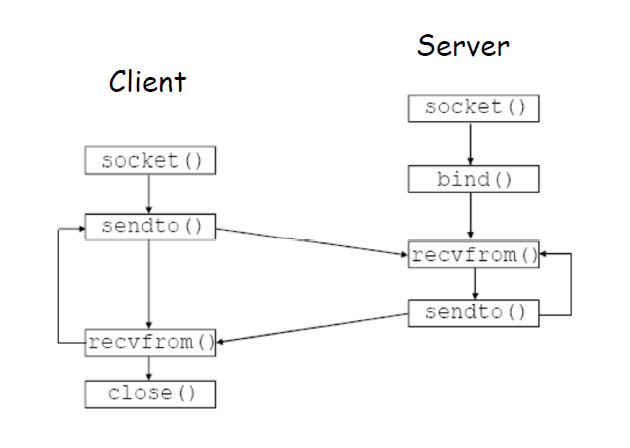
\includegraphics[scale=0.7]{UDP}

\subsubsection*{TCP}

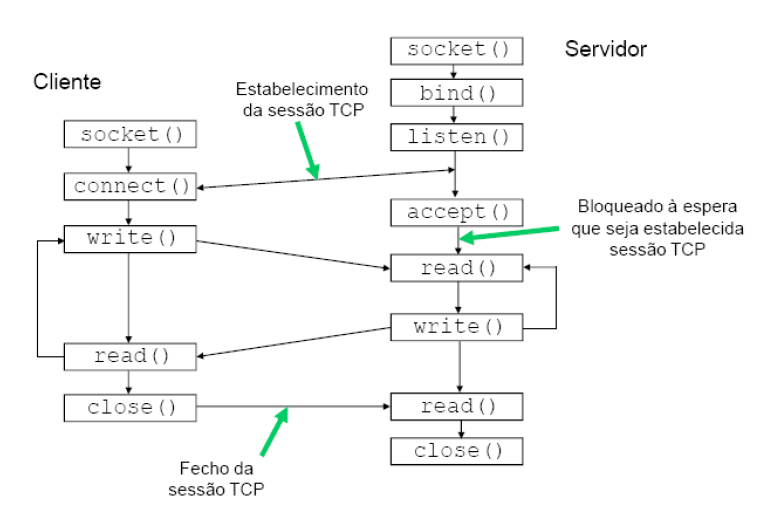
\includegraphics[width=\textwidth]{TCP}

\subsubsection*{TCP vs UDP}

\begin{tabular}{ p{3in} | p{3in} }
    TCP & UDP \\\hline
    read() and write() & sendto() and recvfrom() \\\hline
    Byte stream (no byte is lost) & Messages may be lost \\\hline
    Bytes read with read() may correspond to several write() & Preserves boundary between messages \\\hline
    Bytes written with write() may need to be read with several read() & Each message read with recvfrom() correspond to a single sendto() \\
\end{tabular}

\newpage

\section{Transport Layer}

The Internet's transport layer transports application-layer messages between application endpoints. In the Internet there are two transport protocols, TCP and UDP, either of which can transport application layer messages. TCP provides a connection-oriented service to its applications. This service includes guaranteed delivery of application-layer messages to the destination and flow control (that is, sender/receiver speed matching). TCP also breaks long messages into shorter segments and provides a congestion-control mechanism, so that a source throttles its transmission rate when the network is congested. The UDP protocol provides a connectionless service to its applications. This is a no-frills service that provides no reliability, no flow control, and no congestion control. In this book, we'll refer to a transport-layer packet as a segment.

\subsection{User Datagram Protocol (UDP)}

\begin{itemize}
    \item Um socket UDP é identificado pelo tuplo: (dest IP, dest port)
    \item Quando recebe datagrama UDP, entrega ao socket com esse IP:porto
    \item Sem ligações nem garantias de ordem ou entrega
    \item Sem controlo de congestão
    \item Checksum (opcional):

    Este campo dos segmentos serve para detetar erros num dado segmento transmitido.
    Quando o segmento é enviado, o emissor calcula e guarda a soma dos dois endereços IP enviados (considerados números para ser possível fazer a soma) no campo Checksum.

    Quando o segmento é recebido, o recetor faz a mesma soma e verifica-se se o resultado é igual ao valor que está no campo Checksum.

    Se tiver existido alguma corrupção, ou seja, pelo menos algum bit que tenha sido mal transmitido, a soma dará um valor diferente e então o erro será detetado.
    Se for esse o caso, o pacote é apenas ignorado/dropped (no caso de TCP, o segmento seria antes pedido novamente ao emissor).
    
    Contudo, este sistema continua a não ser muito confiável - podem existir várias combinações de erros que gerem a mesma soma e um erro pode também estar no checksum.
    
    Uma melhoria que se pode fazer é considerar mais valores para o cálculo da soma do checksum, de forma a aumentar a entropia do erro - pode-se, por exemplo, também considerar valores dos cabeçalhos de outras camadas.
\end{itemize}

Headers pequenos, é simples e rápido. Usado para streaming, DNS e SNMP.

\subsection{Reliable Data Transfer (RDT)}

\subsubsection{Stop-and-Wait}

Protocolo de janela deslizante em que a janela de transmissão tem dimensão igual a 1, e janela de receção também tem dimensão igual a 1.

Eficiência de utilização de linha: 
$\displaystyle \frac{\frac{L}{R}}{\frac{L}{R}+RTT}$

\subsubsection{Sliding Window}

Este esquema tem uma "janela" de tempo onde se podem enviar pacotes.\\
Depois dessa janela acabar (ou seja, quando se chegar ao limite de N pacotes pendentes), espera-se pela receção de pelo menos um pacote para poder enviar mais.\\
O ideal seria dimensionar o envio de tal forma que não exista tempo perdido.\\
Contudo, ainda podem existir vários tipos de perdas, como apresentado no RDT 3.0.
Para resolver esses problemas, existem "sub-protocolos".

\subsubsection*{Go-Back-N (GBN)}

Go-back-N é um protocolo em que a janela de transmissão pode ter dimensão $N>1$, mas a janela de receção tem sempre dimensão = 1.

\begin{itemize}
    \item Emissor pode ter até N pacotes enviados à espera de ACK.
    \item ACKs são cumulativos $\left(ACKn \Leftrightarrow  ACK1, ACK2, \cdots, ACKn\right)$
    \item Timer para pacote sem ACK enviado há mais tempo, se expira \textbf{reenvia todos os pacotes seguintes} contidos na janela.
\end{itemize}

\subsubsection*{Selective Repeat (SR)}

Selective Repeat é um protocolo em que a janela de transmissão tem a mesma dimensão da janela de receção.

\begin{itemize}
    \item Emissor pode ter até N pacotes na janela.
    \item ACKs individuais, não cumulativos.
    \item Um timer por pacote unACKed enviado, quando o tempo expira só reenvia esse pacote.
\end{itemize}

\subsection{Transmission Control Protocol (TCP)}

\begin{itemize}
    \item Um socket TCP é identificado pelo tuplo: (src IP, src port, dest IP, dest port)
    \item Há 1 socket por ligação (cliente), cada uma abre um socket novo.
    \item Entrega fiável e ordenada.
\end{itemize}

\newpage

\section{Network Layer}

The Internet's network layer is responsible for moving network-layer packets known as datagrams from one host to another. The Internet transport-layer protocol (TCP or UDP) in a source host passes a transport-layer segment and a destination address to the network layer, just as you would give the postal service a letter with a destination address. The network layer then provides the service of delivering the segment to the transport layer in the destination host. 
\vspace{0.5cm} \\
The Internet's network layer includes the celebrated IP protocol, which defines the fields in the datagram as well as how the end systems and routers act on these fields. There is only one IP protocol, and all Internet components that have a network layer must run the IP protocol. The Internet's network layer also contains routing protocols that determine the routes that datagrams take between sources and destinations. The Internet has many routing protocols. As we saw in Section 1.3, the Internet is a network of networks, and within a network, the network administrator can run any routing protocol desired. Although the network layer contains both the IP protocol and numerous routing protocols, it is often simply referred to as the IP layer, reflecting the fact that IP is the glue that binds the Internet together.

\subsection{Overview of Network Layer}

The primary role of the \textbf{data plane} is to forward datagrams from its input links to its output links. 
\vspace{0.5cm} \\
The primary role of the \textbf{control plane} is to coordinate these local, per-route forwarding actions so that datagrams are ultimately transferred end-to-end, along paths of routers between source and destination.

\subsubsection{Forwarding and Routing: The Data and Control Planes}

The primary role of the network layer is to move packets from the sending host to a receiving host. Thus, there are 2 important network-layer function:

\begin{enumerate}
    \item Forwarding → When a packet arrives at a router's input link, it must move the packet to the appropriate output link. A packet might also be blocked from exiting a router or duplicated and sent over multiple outgoing links. \\
    \textbf{Forwarding is router-local}, and is the key function performed by the data-plane functionality.
    \item Routing → The network layer must determine the path taken by packets as they flow from a sender to a receiver. To do so, the network layer uses multiple routing algorithms. Routing refers to the network-wide.   
    \textbf{Routing is a network-wide process}.
\end{enumerate}

\subsection{}

\subsection{The Internet Protocol (IP)}

\subsubsection{Fragmentation}

\subsubsection{Adressing}

\subsubsection*{Dynamic Host Configuration Protocol (DHCP) [Server Port 67, Client Port 68]}

\begin{itemize}
    \item Mensagens de DHCP são em UDP.
    \item Endereços são emprestados por um tempo finito (lease time).
    \item Após 50\% do lease time, o cliente tenta renovar o IP (\textbf{DHCP Request}). \\
        Se não conseguir, tenta de novo a 85\%.
\end{itemize}

Outras mensagens:

\begin{itemize}[topsep=0pt, itemsep=0pt]
    \item Decline: cliente rejeita oferta
    \item NACK: servidor não consegue satisfazer pedido
    \item Release: cliente informa que já não quer usar endereço
    \item Inform: cliente pede parâmetros extra
\end{itemize}

\subsubsection*{Network Address Translation (NAT)}

\begin{enumerate}
    \item Quando um utilizador da rede privada envia um pacote, o NAT substitui o endereço IP interno do remetente pelo externo, e memoriza o correspondente.
    \item Quando recebe uma resposta o NAT restaura o IP interno.
\end{enumerate}

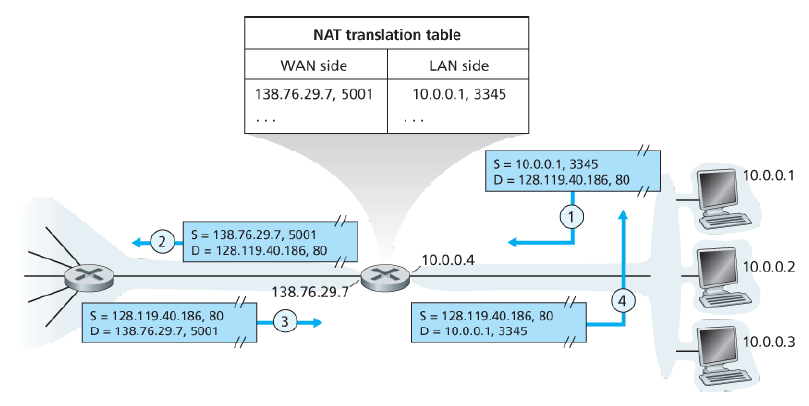
\includegraphics[width=0.9\textwidth]{NAT}

\subsection{Software Defined Network (SDN)}

A abordagem usando SDN para a implementação da camada de rede considera que apenas o plano de dados (\textbf{Data Plane}) é implementado em cada encaminhador.

\subsection{Routing Algorithms}

\subsubsection{Link-State (LS) - Djkstra}

Um encaminhador pode receber mais do que uma cópia de um dado LSP (Link State Packet).

\subsubsection{Distance-Vector (DV) - Bellman-Ford}

\subsection{Broadcast e Multicast}

\subsubsection*{Broadcast}

O objetivo de um Broadcast é enviar um pacote para todos os outros nós da rede.

Contudo, fazer um broadcast pode gerar problemas entre routers. \\

Numa situação em que existe um anel que fará com que o pacote seja enviado de volta para routers que já o receberam - a este problema chama-se Flooding. \\

Para o resolver, um nó só faz broadcast de um pacote se ainda não fez broadcast desse mesmo pacote (Os routers guardam os identificadores dos pacotes) - Controlled Flooding. \\

Outra alternativa seria construir uma Spanning Tree - árvore que cobre todos os routers com o menor número de ligações e sem loops.

\subsubsection*{Multicast}

O objetivo de um Multicast é uma mensagem ser entregue a um grupo de destinatários específico. \\

É usado um endereço IP especial, juntamente com protocolos para gestão local de pertença a um grupo e para a criação de uma árvore de distribuição.

\newpage

\section{Link Layer}

The Internet's network layer routes a datagram through a series of routers between the source and destination. To move a packet from one node (host or router) to the next node in the route, the network layer relies on the services of the link layer. In particular, at each node, the network layer passes the datagram down to the link layer, which delivers the datagram to the next node along the route. At this next node, the link layer passes the datagram up to the network layer. 
\vspace{0.5cm} \\
The services provided by the link layer depend on the specific link-layer protocol that is employed over the link. For example, some link-layer protocols provide reliable delivery, from transmitting node, over one link, to receiving node. Note that this reliable delivery service is different from the reliable delivery service of TCP, which provides reliable delivery from one end system to another. Examples of link-layer protocols include Ethernet, WiFi, and the cable access network's DOCSIS protocol. As datagrams typically need to traverse several links to travel from source to destination, a datagram may be handled by different link-layer protocols at different links along its route. For example, a datagram may be handled by Ethernet on one link and by PPP on the next link. The network layer will receive a different service from each of the different link-layer protocols. In this book, we'll refer to the link-layer packets as
frames.

\subsection{Introduction to the Link Layer}

\subsection{Error Detection and Correction Techniques}

Os dados, por diversos motivos, podem sofrer erros de transmissão, fazendo com que um ou mais bits venham trocados.

Para detetar esses erros, existem várias formas:

\subsubsection{Parity Checks}

Forma antiga de detetar erros.

No fim da transmissão, era acrescentado um bit que dependia do número de bits totais da mensagem:

\begin{itemize}
    \item Se o número de bits fosse par, colocava-se um 0;
    \item Se o número de bits fosse ímpar, colocava-se um 1.
\end{itemize}

Não é uma forma muito boa pois não deteta um número par de erros.

\subsubsection{Cyclic Redundancy Check (CRC)}

Muito usado atualmente. É feita uma operação matemática, usando divisão de polinómios.

\begin{itemize}
    \item Para gerar mensagem com CRC: \\[4pt]
        Dada uma mensagem: $1001\ 1010$ \\
        Dado um polinómio gerador: $x^3+x^2+1 \ \rightarrow\  1101\ (n=3)$
        \begin{enumerate}
            \item Fazemos shift left da mensagem correspondente ao grau do polinómio ($n$): \\
            $1001\ 1010 \ \rightarrow\  100\ 1101\ 0000$
            \item Fazemos a divisão da mensagem shiftada pelo polinómio gerador, obtendo um resto: \\
            $100\ 1101\ 0000 \div 1101 = quociente + 101$
            \item A mensagem que será transmitida é a soma da mensagem shiftada com o resto: \\
            $100\ 1101\ 0000 + 101 = 100\ 1101\ 0101$ 
        \end{enumerate}
    \item Para verificar se a mensagem recebida tem erros: \\[4pt]
        Dada uma mensagem recebida: $10\ 1010\ 0111$ \\
        Dado um polinómio gerador: $x^3+x^2+1 \ \rightarrow\  1101$
        \begin{enumerate}
            \item Fazemos a divisão da mensagem recebida pelo polinómio gerador, obtendo um resto: \\
            $10\ 1010\ 0111 \div 1101 = quociente + 001$
            \item Se o resto da divisão for diferente de zero significa que foi detetado um erro.
        \end{enumerate}
\end{itemize}




\subsection{Multiple Access Links and Protocols}

Quando é feito um broadcast FF:FF:FF:FF:FF:FF, este é partilhado por todos os membros da rede. Isto implica que o canal possa sofrer colisões muito facilmente, bastando que um nó receba dois ou mais sinais ao mesmo tempo. \\

Protocolos Multiple Access Control - algoritmos distribuídos que determinam como é que os nós partilham um canal, ou seja, quando é que um dado nó pode transmitir.

Existem vários protocolos que implementam o acesso de formas diferentes:

\subsubsection{Channel Partitioning Protocols}

\begin{itemize}
    \item Dividir o canal em "pedaços" menores (intervalos de tempo, frequências, códigos, ...);
    \item Alocar um pedaço para o nó para uso exclusivo.
\end{itemize}

\subsubsection*{Frequency Division Multiple Access (FDMA)}

Neste tipo de particionamento, o espectro de canal é dividido em faixas de frequência. Assim, é atribuída a cada estação uma faixa de frequência fixa mas o tempo de transmissão não utilizado nas faixas de frequência não é aproveitado.

\subsubsection*{Time Division Multiple Access (TDMA)}

O acesso ao canal é feito em rondas. É atribuído a cada host uma fatia temporal em cada ronda. Também aqui, o tempo não utilizado não é aproveitado.

\subsubsection*{Code Division Multiple Access (CDMA)}

Cada utilizador tem acesso à frequência completa, durante todo o tempo.
São usados diferentes códigos para distinguir os utilizadores.

\subsubsection{Dynamic Allocation Protocols (Taking-Turns)}

\begin{itemize}
    \item Os nós tomam a vez (mas os nós com mais dados para enviar podem transmitir com mais frequência);
\end{itemize}

\subsubsection*{Poll / Select}

Um computador central controla a atividade dos outros.

\subsubsection*{Token Passing}

Um token que dá a permissão de transmissão é passado entre os hosts.

Quando um host acaba de transmitir, passa o token para outro host.\\

Esta medida não é ideal se não existir muito tráfego, pois existe dependência que os hosts transmitam mensagens.

\subsubsection{Random Access Protocols}

\begin{itemize}
    \item O canal não é dividido, logo permite colisões;
    \item É possível recuperar das colisões.
\end{itemize}

\subsubsection*{ALOHA}

É um protocolo simples que não tem sincronização. \\
Existe uma colisão se duas ou mais tramas se sobrepuserem, sendo programada uma retransmissão para um instante futuro aleatório.

\subsubsection*{Slotted ALOHA}

Igual ao protocolo anterior, mas o tempo é dividido em slots temporais do mesmo tamanho. \\
Os nós só podem começar a transmitir no início de um slot.

\subsubsection*{Carrier Sense Multiple Access (CSMA)}

Baseia-se em não causar interrupções:

\begin{itemize}
    \item Se o canal estiver calado, transmite a trama inteira;
    \item Se o canal estiver ocupado, adia a transmissão.
\end{itemize}

Contudo, ainda podem existir colisões devido ao tempo de propagação, o que implica que toda a transmissão de um pacote tenha que ser descartada.

\subsubsection*{CSMA with Collision Detection (CSMA$\backslash$CD)}

Versão aprimorada do protocolo anterior, onde consegue detetar colisões mais rapidamente. Ao ser detetada uma colisão, as transmissões são imediatamente abortadas, reduzindo a ocupação do canal.

\subsection{Summary of MAC Protocols}

Channel Partitioning Protocols:

\begin{itemize}[topsep=0pt, itemsep=0pt]
    \item Eficientes com uma carga alta e constante de todos os nós;
    \item Ineficientes em cargas baixas ou desequilibradas.
\end{itemize}

Dynamic Allocation Protocols (Taking-Turns):

\begin{itemize}[topsep=0pt, itemsep=0pt]
    \item Compartilham o canal de forma eficiente e justa em cargas altas;
    \item Baixa carga: ineficiente, pois os nós ativos precisam esperar pelos nós sem/com pouca atividade para "passarem a vez";
\end{itemize}

Random Access Protocols:

\begin{itemize}[topsep=0pt, itemsep=0pt]
    \item Eficientes em carga baixa: um único nó pode utilizar unicamente o canal;
    \item Carga alta: sobrecarga de colisão.
\end{itemize}

\subsection{Switched Local Area Networks}

\subsubsection{Link-Layer Addressing and ARP}

\subsubsection*{MAC Addresses}

Estes endereços têm propósitos diferentes dos endereços IP: os endereços MAC têm um propósito mais local enquanto que os endereços IP têm um contexto mais geográfico. 

O que cria esta distinção é o facto de os endereços MAC serem intrínsecos das placas de rede, ou seja, são como uma fingerprint; Já os endereços IP podem ser alterados facilmente e é possível ser construído um sistema e uma divisão hierárquica da sua distribuição, através das máscaras de rede. \\

Para um dado endereço MAC, os três primeiros bytes identificam o fabricante enquanto que os os três últimos bytes identificam o equipamento. \\

Nestes endereços também é possível ser feito um broadcast, fazendo-o para o endereço \\ FF:FF:FF:FF:FF:FF. Ao enviar um pacote para esse endereço, esse pacote será reencaminhado para todos os hosts da rede local.

\subsubsection*{Address Resolution Protocol (ARP)}

O router precisa de saber o endereço MAC correspondente ao endereço IP recebido.
Para tal, usa-se o protocolo ARP - Address Resolution Protocol:

\begin{enumerate}
    \item O router faz um ARP Request, ou seja, um broadcast, enviando para o endereço FF:FF:FF:FF:FF a pergunta: Quem tem este endereço IP?
    \item O host com o endereço IP responde com o seu endereço MAC.
\end{enumerate}

De forma a não se estarem sempre a repetir estes pedidos, os hosts guardam numa tabela (tabela ARP), o mapeamento entre endereço IP e endereço MAC - (endereço IP, endereço MAC, TTL).

\subsubsection{Ethernet}

\subsubsection{Link-Layer Switches}

\subsubsection*{Self-Learning}

Switches are self-learning, meaning the switch table is built automatically, dynamically and autonomously.

\begin{enumerate}
    \item The switch table is initially empty.
    \item For each incoming frame received on an interface, the switch stores in its table: \\
        \begin{tabular}[t]{ | c | c | c | }
            \hline
            MAC Address & Interface & Current time \\\hline
            E6-E9-00-17-BB-4B & 1 & 00:01 \\\hline
        \end{tabular}
    \item The switch deletes an address in the table if no frames are received with that address as the source address after some time (\textbf{aging time}).
\end{enumerate}

\subsubsection*{Spanning-Tree Protocol (STP)}

\begin{itemize}
    \item Establishes a root node called the root bridge.
    \item Constructs a topology that has one path from/to every network node.
    \item Resulting tree originates from the root bridge.
    \item Redundant links that are not part of the shortest path are blocked.
\end{itemize}

\subsubsection*{Bridge Protocol Data Unit (BPDU)}

Convention for Conf-BPDUs: Root ID . Root Path Cost . Bridge ID \\\newline
A configuration $C_1$ is said to be better than $C_2$ if (ordered by decreasing importance):

\begin{enumerate}[topsep=0pt, itemsep=0pt]
    \item $C_1$ Root ID is lower than that of $C_2$.
    \item $C_1$ Root Path Cost is lower than that of $C_2$.
    \item $C_1$ Bridge ID is lower than that of $C_2$.
    \item $C_1$ Port ID is lower than that of $C_2$.
\end{enumerate}

\subsubsection{Virtual Local Area Networks (VLANs)}

Existem switches que suportam o uso de VLANs - Virtual LANs, ou seja, permitem configurar redes virtuais para as suas portas.\\

As VLANs têm algumas vantagens:

\begin{enumerate}
    \item dividem a rede em partes, reduzindo o domínio de broadcast o que, consequentemente, aumenta a bandwidth pois as mensagens não são enviadas para portas desnecessárias;
    \item adicionam segurança, pois hosts em diferentes VLANs não conseguem comunicar entre si diretamente;
\end{enumerate}

Para as VLANs comunicarem entre si, isso é feito através de routing (pelos Routers).

\subsection{Wireless [802.11]}

\subsubsection{Architecture}

\subsubsection{MAC Protocol}

\subsubsection*{Carrier Sense Multiple Access with Collision Avoidance (CSMA/CA)}

Este algoritmo é bastante similar ao básico CSMA. O que difere dele é que, para além de esperar que o canal fique livre, ainda espera um tempo aleatório depois do canal se libertar, e esse tempo só é descontado quando o canal está livre.
Assim, o "sortudo" que teve o tempo menor começa a transmitir e os outros voltam a ficar à espera que o canal fique livre.

Depois de uma transmissão, o AP devolve um ACK para confirmar o sucesso da transmissão. Isto ajuda a resolver o problema do terminal escondido - porém não o resolve de todo pois podem haver tempos em que o início das transmissões coincide.

Para resolver isto, surgiu a variante com RTS-CTS.

\subsubsection*{CSMA/CA com Request-To-Send e Clear-To-Send (RTS-CTS)}

Esta variante consiste numa reserva do canal - o emissor, no lugar de começar a sua transmissão imediatamente, envia antes um pedido de reserva do canal.
Desta forma, o AP irá-lhe reservar o canal e dar-lhe um OK, fazendo broadcast de um CTS com a informação de quem vai emitir.
Assim, um outro host que não oiça o emissor, ouvirá certamente o AP e não irá transmitir.

Se tiver existido uma colisão nesse pedido, esta terá um impacto muito reduzido, pois foi apenas transmitido um pacote.

\end{document}
